\section{Network Structure for Hourglass-type DenseReg}
\begin{figure}[!h]
\centering
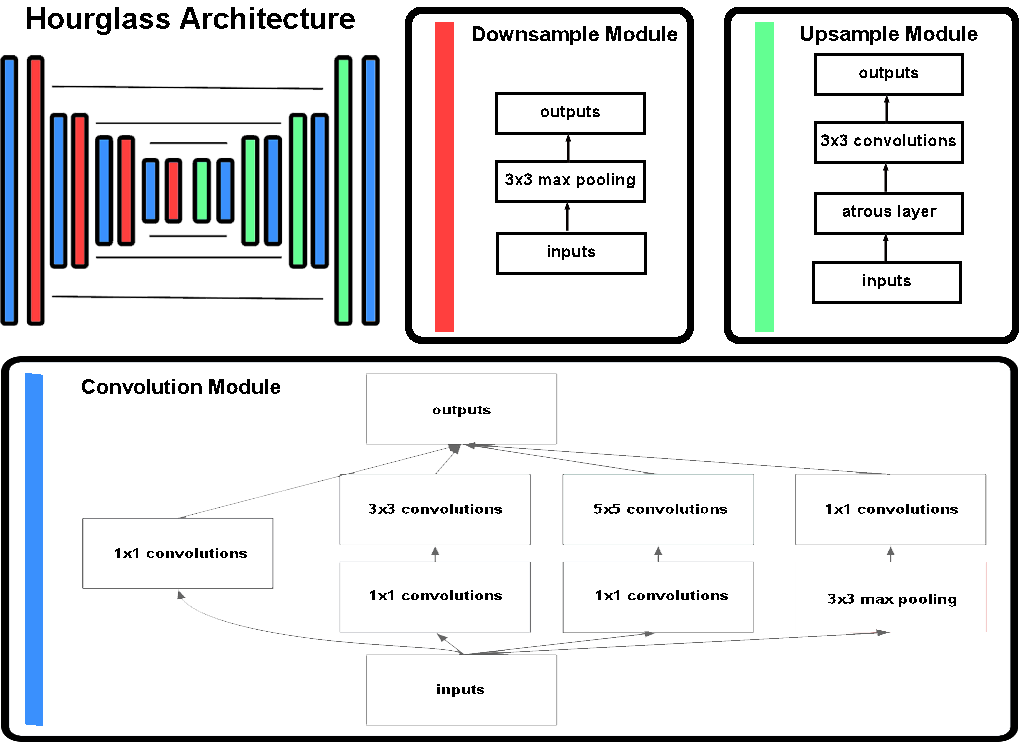
\includegraphics[width=\linewidth]{Figures/hourglass_archietecture}
\caption{Hourglass architecture with inception-v2 module.}
\label{fig:hourglass_arch}

\end{figure}

Figure\ref{fig:hourglass_arch} demonstrated the hourglass architecture \cite{newell2016stacked} we used with some modifications. The network is consisted by three type of modules: 1) the convolution module (blue), 2) the down sampling module (read) and 3) the up sampling module. The whole hourglass is constructed with a list convolution modules at 4 different scales with corresponding down/up sampling modules between those convolution modules. There are also bilateral connection between layers of the same scale. The composition of each type of modules are shown in the figure too. The down sampling module is just a $3\times3$ max pooling layer and the up sampling module is using a $3\times3$ atrous layer following by a $3\times3$ convolution layer. The majority of the parameters are lies in the convolution module. The original hourglass uses a chain of 3 convolution layers as its convolution module, while replacing that with the inception-v2 type module shows slight improvement on body pose estimation and obvious improvement on training speed.